\documentclass[a4paper,12pt]{article}
\usepackage[dvipsnames]{xcolor}
\usepackage[skip=10pt plus1pt, indent=0pt]{parskip}
\usepackage{graphicx} % Required for inserting images
\usepackage{listings}
\usepackage{amsmath}
\usepackage{float}
\usepackage{geometry}
 \geometry{
 a4paper,
 left=25mm,
 right=25mm,
 top=30mm,
 bottom=30mm,
 }
 \usepackage{hyperref}
\hypersetup{
    colorlinks=true,
    linktoc=all,
    linkcolor=black,
}

\title{Riconoscimento di caratteri scritti a mano con rete neurale convoluzionale}
\author{Christian Pozzoli 29678A}
\date{Settembre 2025}

\begin{document}
\lstset{
language=Python,
basicstyle=\fontfamily{pcr}\footnotesize,
comment=[l]{//},
commentstyle=\color{OliveGreen}\ttfamily,
keywordstyle=\color{NavyBlue}\bfseries,
ndkeywordstyle=\bfseries
}
\maketitle
\renewcommand*\contentsname{Indice}
\tableofcontents
\newpage

\section{Introduzione}
\subsection{Riconoscimento ottico dei caratteri}
Il concetto di riconoscimento dei caratteri, in particolare il riconoscimento ottico, è un campo di ricerca molto attivo nell'intelligenza artificiale, nella visione artificiale e nel riconoscimento dei pattern. Nonostante le sue numerose e diffuse applicazioni in sistemi moderni, il concetto di OCR (optical character recognition) si è sviluppato all'inizio del XX secolo, inizialmente come strumento di accessibilità, soprattutto per supportare le persone ipovedenti. Le prime tecniche di riconoscimento si basavano sull'analisi delle componenti chimiche della stampa, o sullo sfruttamento del contrasto luminoso tra il nero del carattere stampato e la carta di colore chiaro. Tuttavia, il riconoscimento dei caratteri ha sempre dovuto affrontare sfide significative: la varietà di font, la qualità della stampa, le deformazioni dei caratteri e la gestione del rumore rappresentavano ostacoli da superare per garantire una lettura accurata.

Nonostante queste difficoltà, la necessità di leggere e interpretare il testo ha continuato a crescere, portando allo sviluppo di tecniche più sofisticate. Con il tempo, con l'incremento dei contenuti digitali e la conseguente evoluzione delle esigenze, il riconoscimento digitale ha assunto la preminenza, diventando indipendente dalla fonte e sempre denominato OCR. Questo avanzamento ha permesso di digitalizzare documenti scansionati, di interpretare il testo presente in immagini e video, e di automatizzare processi che prima richiedevano l'intervento umano. Pur mantenendo la sigla OCR, la tecnologia è entrata in un ciclo continuo di miglioramento, sfruttando l'intelligenza artificiale e il deep learning per aumentare la precisione e l'affidabilità del riconoscimento.

\subsection{Obiettivo}
L'obiettivo del progetto è quella di costruire una rete neurale capace di riconoscere i caratteri scritti a mano.
È quindi necessario strutturare una rete neurale capace di apprendere da una dataset le caratteristiche delle singole letterecon l'obiettivo di riconoscerle con alta attendibilità anche se di origine esterna all'insieme dei dati utilizzati per l'allenamento.
Sarà, quindi, sviluppato anche un tool per permettere a un utente di disegnare un carattere da fare riconoscere alla rete neurale costruita.

\subsection{Strumenti}
Lo sviluppo della rete neurale è realizzato in Python, utilizzando Jupyter Notebook come ambiente di lavoro interattivo per gestire in modo ordinato le fasi di analisi, sperimentazione ed esecuzione del codice, oltre alla visualizzazione dei risultati.

Le librerie NumPy e Pandas sono impiegate per la gestione e l'elaborazione efficiente dei dati, mentre Matplotlib supporta la creazione di grafici e visualizzazioni utili all'analisi delle prestazioni del modello.
La libreria OpenCV è utilizzata per il pre-processamento e la manipolazione delle immagini, operazioni fondamentali per l'addestramento.
La costruzione e l'addestramento della rete neurale sono realizzati con TensorFlow e Keras come framework principali. Infine, Tkinter permette lo sviluppo di un'interfaccia grafica semplice, attraverso cui l'utente può disegnare un carattere e sottoporlo direttamente al modello per il riconoscimento.

\section{Reti neurali convoluzionali}
Con l'obiettivo di sviluppare un agente capace di riconoscere caratteri scritti, ci si confronta con il problema dell'elaborazione di immagini, in quanto il dato da classificare si presenta come una matrice di pixel (in questo caso in scala di grigi).
Una tipologia di rete neurale particolarmente adatta a riconoscere elementi a partire da una rappresentazione visiva è la rete neurale convoluzionale (CNN), la cui architettura si ispira alla corteccia visiva degli animali in cui i neuroni sono organizzati in modo da rispondere a regioni parzialmente sovrapposte che compongono l'intero campo visivo.
Nel mondo biologico, il modo in cui i neuroni reagiscono e si dispongono lungo il campo visivo corrisponde, in termini matematici, all'operazione di convoluzione.
Tale operazione, ampiamente utilizzata anche nella teoria dei segnali, consiste nel calcolare l'integrale del prodotto di due funzioni, dopo averne riflessa una rispetto all'asse $y$ e traslata.
Nel caso di un'immagine, la convoluzione viene applicata a ciascun pixel come prodotto scalare tra una matrice, chiamata filtro (o kernel), e la porzione dell'immagine su cui essa si sovrappone (nel deep learning si utilizza spesso una variante chiamata cross-correlation, che evita il passaggio di riflessione).
Questa operazione permette alla rete neurale di estrarre delle feature dall'immagine, in modo da poter riconoscere i contenuti e categorizzare i dati.
I filtri rappresentano quindi i pesi di un layer convoluzionale e vengono ottimizzati durante l'addestramento per catturare le caratteristiche più utili al compito.
Solitamente i layer convoluzionali sono intervallati da dei layer di pooling che riducono la dimensione spaziale dell'immagine, aggregando regioni adiacenti (con, ad esempio, logice di media o di massimo). Questa riduzione abbassa il costo computazionale dei livelli successivi, riduce il rischio di overfitting e aumenta il campo recettivo della rete.
Nei primi livelli vengono individuate feature locali e specifiche (bordi, texture), mentre con il pooling e la progressione degli strati la rete impara rappresentazioni sempre più astratte e globali, capaci di riconoscere le strutture e i componenti principali del soggetto nell'immagine.

\section{Implementazione}
Conoscendo il concetto di rete neurale convoluzionale, è possibile progettare e realizzare una rete profonda (deep network) capace di svolgere il compito di riconoscimento descritto in precedenza. La costruzione di una rete di questo tipo non si limita alla definizione della sua architettura generale, ma richiede anche una serie di decisioni riguardanti sia la scelta dei parametri e degli iperparametri, sia le modalità di implementazione e ottimizzazione del modello.
Gli iperparametri comprendono, ad esempio, il numero di strati convoluzionali e completamente connessi, la dimensione dei filtri (kernel size), il passo di convoluzione (stride), la funzione di attivazione, la dimensione dei batch, la velocità di apprendimento (learning rate) e le tecniche di regolarizzazione. Ognuno di questi elementi può influenzare in maniera significativa non solo l'accuratezza finale del modello, ma anche il tempo di addestramento, l'uso delle risorse di calcolo e la capacità della rete di generalizzare su dati non visti.
Nella fase di sviluppo è quindi fondamentale bilanciare prestazioni ed efficienza, evitando di progettare un'architettura eccessivamente complessa che possa portare a problemi di overfitting, oppure troppo semplice da non riuscire a catturare le caratteristiche rilevanti dei dati.
Nei paragrafi seguenti verranno illustrate le scelte progettuali adottate.

\subsection{Dati}
Per addestrare la rete neurale è necessario disporre di una grande quantità di dati; in questo caso si tratta di più di 370000 lettere maiuscole scritte a mano, con differenti tratti e stili, in modo da addestrare la rete a riconoscere i caratteri dalle forme, dalle curve e dai tratti che li compongono, piuttosto che dai singoli pixel occupati.
Il dataset è in formato CSV ed è composto da 372450 righe (numero di lettere) e da 785 colonne. La prima colonna rappresenta l'etichetta (la posizione della lettera nell'alfabeto), con valori compresi tra 0 e 25; le successive colonne contengono l'elenco dei pixel, cioè un elenco di 784 valori da 0 a 255 che rappresentano un'immagine di dimensione $28\times28$ in scala di grigi.
Per poter utilizzare questi dati è necessario modificare la loro struttura in memoria in base alle esigenze.

\begin{figure}
    \centering
    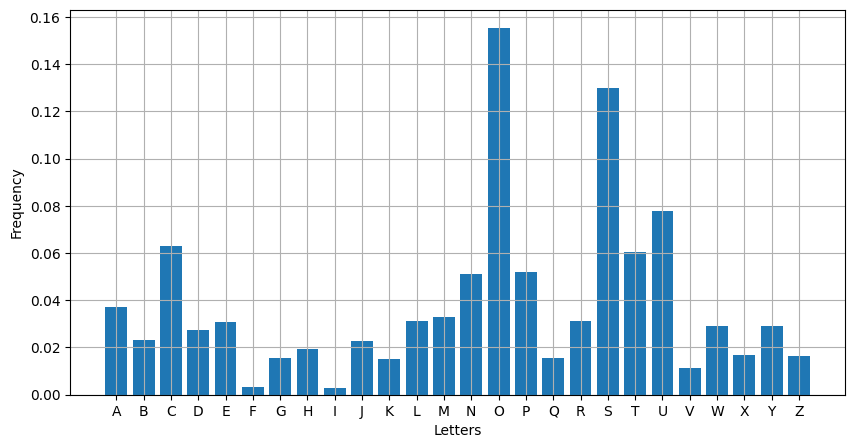
\includegraphics[width=1\linewidth]{images/letters_frequency.png}
    \caption{Frequenza delle lettere nel dataset}
    \label{letters_frequency}
\end{figure}

Come prima operazione è utile aggiungere una colonna iniziale che rappresenti il numero progressivo del dato, in modo da poterlo usare come \texttt{id} del singolo campione e risalire così all'immagine corrispondente. Questo risulta molto utile, ad esempio, quando si vuole individuare uno specifico dato critico che la rete non è riuscita a riconoscere. Questo passaggio è necessario in quanto la prossima trasformazione è la randomizzazione dell'intero dataset. Inizialmente i dati sono ordinati per etichetta dalla A alla Z; utilizzare i dati in questo ordine porterebbe la rete a:
\begin{itemize}
    \item incorrere in overfitting sulle singole lettere anziché imparare pattern generali;
    \item apprendere più lentamente;
    \item avere difficoltà nella ricerca di un minimo globale;
    \item dimenticare le prime lettere apprese.
\end{itemize}
Pertanto, si randomizza prima l'ordine delle righe e successivamente si separano gli indici e le etichette dal dataset vero e proprio.
Oltre a questa suddivisione in colonne, la fase di addestramento richiede anche una suddivisione in righe, con l'obiettivo di ottenere due insiemi di dati: i dati di training, utilizzati per l'addestramento, e i dati di test, utilizzati come controllo sull'andamento dell'errore per evitare overfitting. Una percentuale comune per questo tipo di suddivisione è 80\% di dati training e 20\% dati di test.
Infine, per la rappresentazione del dato e l'elaborazione da parte della rete, anziché un singolo vettore, è bene disporre i dati secondo una matrice $28\times28$.

\begin{figure}
    \centering
    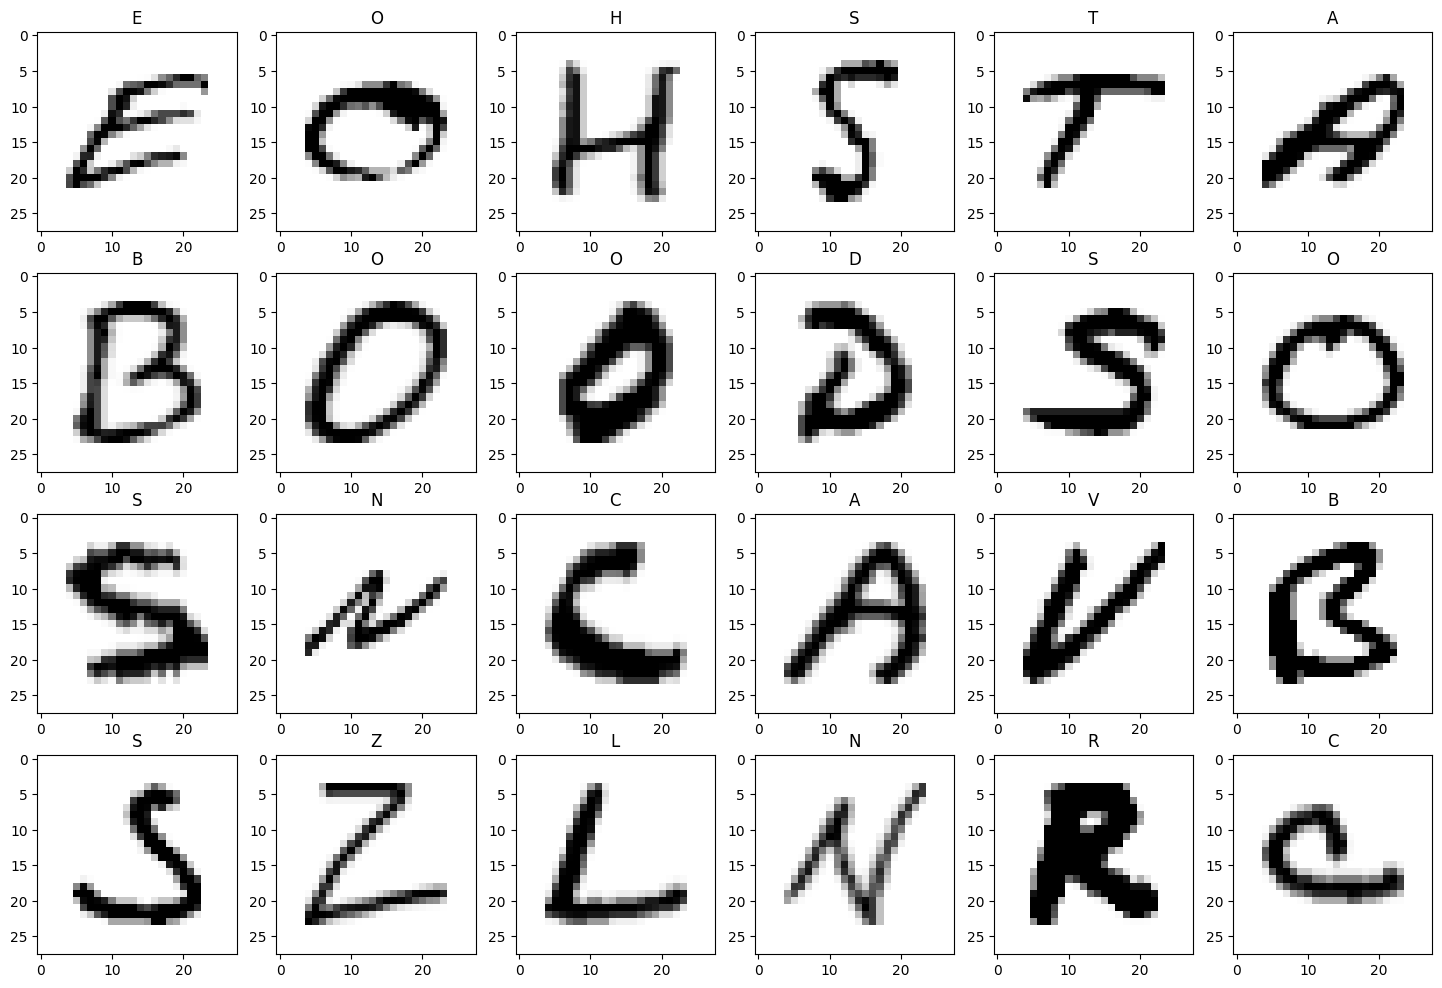
\includegraphics[width=1\linewidth]{images/some_letters.png}
    \caption{Visualizzazione di alcune lettere}
    \label{some_letters}
\end{figure}

\subsection{Layer}
\subsubsection{Pooling}
\subsection{Funzioni di attivazione}
\subsection{Ottimizzatori}

\section{Risultato}
\subsection{Step intermedi}

\section{Conclusioni}
\subsection{Limiti}

\end{document}